\documentclass[tikz, border = 2mm]{standalone}
% \usepackage{kompendium-figurer}
\usepackage{pgfplots}
\usepgfplotslibrary{fillbetween}

    \pgfkeys{/pgfplots/Delta Style/.style={
		    % scale only axis,
		    grid=major,
		    axis equal,
		    grid style={dashed, gray!30}, %Uncomment these lines for no grid
		    axis lines=middle,
		    inner axis line style={=stealth}, %Arrow type
        ultra thick,
		    xlabel={\large $x$},
		    ylabel={\large $y$},
        cycle list = {black,black!70,black!40,black!10} %Plot colors cycle in grayscale
      }}

    \pgfplotsset{
        % use this `compat' level or higher to use the LUA backend for calculation
        % (--> speed improvement)
        compat=1.12,
        % declare your function here ...
        /pgf/declare function={
            f(\x) = 2*\x+1;
        },
        /pgf/declare function={
            y(\y) = 0.5*(\y-1);
        },
    }

\begin{document}
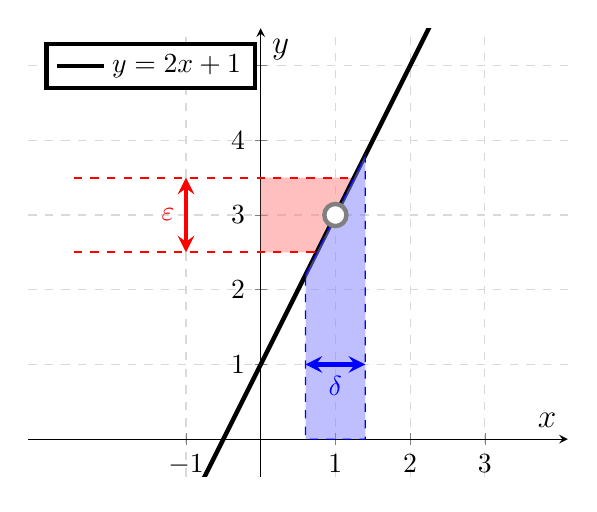
\begin{tikzpicture}
  \def\e{0.5}
  \def\ea{3-\e}
  \def\eb{3+\e}
  
  \def\d{0.4}
  \def\da{1-\d}
  \def\db{1+\d}
  
  \begin{axis}[
    Delta Style,
    legend pos =north west,
    ytick={-1,0,...,8},
    xtick={-1,0,...,3},
    ymin=-0.5,
    ymax=5.5,
    xmin=-1.5,
    xmax=2.5,
		]
    % Filling
    \addplot[name path=plot,ultra thick,samples=100,domain= -10:10] {f(x)};
    \addlegendentry{$y=2x+1$}
    \path[name path=yaxis](current axis.below origin)-- (current axis.above origin);

    \addplot[red!50, fill opacity=0.5] fill between[
    of=yaxis and plot,reverse=false,
    soft clip={domain y = \ea:\eb},
    ];

    \addplot[domain=\da:\db,blue,dashed, fill=blue!50, fill opacity=0.5] {f(x)}\closedcycle;
  
        \addplot[color=gray,fill=white,only marks,mark size = 4pt] coordinates {(1,3)};

        \addplot[dashed,thick,red, domain=-2.5:y(\ea)] {\ea};
        \addplot[dashed,thick,red, domain=-2.5:y(\eb)] {\eb};

        \draw[ultra thick, red, stealth-stealth] %
        (axis cs: -1, \ea) -- node[left] { $\varepsilon$ } (axis cs:-1, \eb);
        \draw[ultra thick, blue, stealth-stealth] %
        (axis cs: \da, 1) -- node[below] { $\delta$ } (axis cs: \db, 1);
		\end{axis}
	\end{tikzpicture}
\end{document}